\chapter{Conclusion}\label{cap:conclusions}
\intro{
    In this chapter we will present the conclusions of our work, the results obtained and the future developments of the project.
}
\section{Goals achieved}
In the following table we will show the goals achieved and the ones that are still in progress. (Refer to table~\ref{tab:goals} for the meaning of the acronyms)
\begin{table}[H]
    \caption{Reached Goals}\label{tab:reach-goals}
    \centering
    \begin{tabular}{|c|c|}
        \hline
        \textbf{Code} & \textbf{Status}\\
        \hline
        M1 & Achieved\\
        \hline
        M2 & Achieved\\
        \hline
        M3 & Achieved\\
        \hline
        D1 & Achieved\\
        \hline
        D2 & Not Achieved\\
        \hline
        D3 & Achieved\\
        \hline
        O1 & Achieved\\
        \hline
        O2 & Partially Achieved\\
        \hline
    \end{tabular}
\end{table}
All the goals marked as achieved are fully implemented and tested.
\textbf{D2} was tested but the results were not satisfactory, so it was decided to not implement it.
\textbf{O2} was partially implemented, the model and the technologies are too young to be used in a manufacturing production environment.
\subsection{CAD to GAN}\label{subsec:cad-to-gan}
\begin{figure}
    \centering
    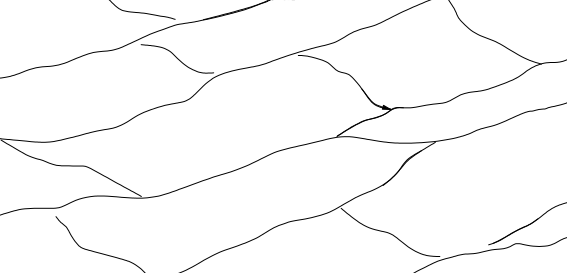
\includegraphics[width=0.50\textwidth]{images/cad-to-gan/mask}
    \caption{CAD drawing}\label{fig:mask}
\end{figure}
The transformation from a \gls{cadg} file (ref.~\ref{fig:cad-to-gan}) to the final image representation of a slab involved a series of steps aimed at producing a realistic output. 
The objective was not only to preserve the visual characteristics and details of the \gls{cadg} file's outlines but also to create an image that closely resembled a real slab.

Initially, the \gls{cadg} file was converted into an image format, ensuring that the geometric information was accurately represented. 
This conversion facilitated further processing and manipulation of the \gls{cadg} data.

Following the conversion, the image file was divided into smaller portions, each conforming to the input requirements of the \gls{gang} model, with dimensions set at 256 X 256 pixels. 
By segmenting the image, we enabled the \gls{gang} model to process the data efficiently and generate high-quality results.

Subsequently, the \gls{gang} model was applied to each segment, generating a set of individual images. 
These images captured various characteristics and textures associated with slabs, enhancing the realism of the final output.

To create a cohesive representation of the slab, the individual images were carefully arranged and merged together. 
Through meticulous alignment and blending techniques, the resulting composite image closely resembled a genuine slab, incorporating the appearance and details that one would expect from a real-world sample.

By employing this comprehensive transformation pipeline, the \gls{cadg} file was successfully translated into an input image that, when combined and processed by the \gls{gang} model, resulted in a realistic depiction of a slab. 
This process ensured that the final image conveyed the visual attributes and authenticity typically associated with real slabs.

\begin{figure}
    \centering
    
\includegraphics[width=0.50\textwidth]{images/cad-to-gan/result}
    \caption{Result IMG}\label{fig:cad-to-gan}
\end{figure}

\subsubsection{Challenges}\label{subsec:issues}
The output obtained, as depicted in Figure~\ref{fig:cad-to-gan}, reveals visible imperfections, notably the noticeable line between the two merged images. 
This discrepancy arises from generating the image components separately and subsequently merging them, resulting in imperfect alignment. 
While the main veins align reasonably well, the background color fails to exhibit proper uniformity.

During the internship period, significant efforts were dedicated to addressing this issue by enhancing the model's quality. 
However, the achieved results fell short of expectations. To overcome this challenge, it was proposed to generate the entire image in a single iteration. 
Regrettably, the current model does not support this approach, as it would necessitate increased computational resources and time, rendering it unfeasible within the constraints of the internship period.
\section{Hourly summary}
As per the initial work plan, a total of 320 hours were allocated for the project, with an intentional overestimation of hourly commitments to account for potential absences or unforeseen circumstances. 
The purpose of this buffer was to ensure that the project could be completed comfortably within the allocated time frame.
Upon completion of the project, it was found that the actual total hours invested in the project amounted to 300 hours. 
This indicates that the project was completed within the expected time frame, demonstrating a commendable consistency between the planned and actual hours spent.
The adherence to the projected hour count is indicative of effective project management and efficient utilization of resources. 
The slight underestimation of hours compared to the initial estimate further highlights the successful management of time and effort throughout the project duration.
\section{Acquired knowledge}
During the course of the project, I had the opportunity to acquire valuable managerial and interpersonal skills while working in a collaborative research team comprising three individuals. 
Additionally, I delved into fields of AI that were previously unfamiliar to me, gaining comprehensive knowledge not only about AI in general but also, in particular, about Generative Adversarial Networks (GANs).

One of the significant areas of growth was in the realm of project management. Collaborating with team members allowed me to enhance my ability to coordinate tasks, set goals, and allocate resources effectively. 
I also developed strong communication and teamwork skills through regular interactions, discussions, and brainstorming sessions. 
This experience highlighted the importance of clear and concise communication, active listening, and the ability to work harmoniously towards a common objective.

In terms of technical knowledge, I embarked on an exploration of AI fields that were previously unfamiliar to me. 
This journey broadened my understanding of AI principles, methodologies, and techniques. 
More specifically, I gained in-depth knowledge about Generative Adversarial Networks (GANs) and their applications in various domains. 
This encompassed comprehending the underlying architecture, training procedures, and optimization techniques related to GANs.

Furthermore, I expanded my expertise in Python libraries specifically tailored for computer vision and AI applications. 
Through hands-on experience, I became proficient in utilizing popular libraries such as TensorFlow, PyTorch, and OpenCV.\@
These libraries proved instrumental in implementing computer vision algorithms and working with AI models efficiently.

In summary, this project provided me with valuable insights and knowledge in both managerial and technical domains. 
The collaborative research environment fostered the development of essential interpersonal skills, while the exploration of unfamiliar AI fields and the utilization of Python libraries enhanced my technical proficiency. 
The acquired knowledge and skills from this project will undoubtedly contribute to my future endeavors in the field of AI and beyond.
\section{Personal evaluation.}
My internship experience has been truly invaluable and has provided me with a multitude of learning opportunities and personal growth. 
Throughout the duration of the internship, I have had the chance to work in a professional setting, applying the knowledge and skills I acquired during my studies.

One aspect of the internship that I found particularly rewarding was the exposure to real-world scenarios and challenges. This allowed me to bridge the gap between theory and practice, gaining a deeper understanding of how concepts and principles are applied in a professional context. 
The hands-on experience has enhanced my problem-solving abilities and critical thinking skills, enabling me to approach tasks with a more practical and solution-oriented mindset.

Moreover, the internship provided me with a chance to collaborate with a diverse team of professionals. This collaborative environment allowed me to learn from others, exchange ideas, and contribute to meaningful projects. 
Working alongside experienced colleagues has not only expanded my technical knowledge but has also helped me refine my interpersonal skills such as effective communication, teamwork, and adaptability.

also appreciated the mentorship and guidance provided by my supervisor throughout the internship. 
Their support and feedback have been instrumental in my growth and development. They provided valuable insights, challenged me to think outside the box, and encouraged me to take ownership of my work. 
This guidance has not only enhanced my technical skills but has also boosted my confidence in tackling complex tasks and projects.

In terms of personal growth, this internship has helped me develop a greater sense of professionalism and work ethic. It has instilled in me a strong sense of responsibility, time management, and the importance of meeting deadlines. 
The experience has also reinforced my passion for the field and has motivated me to continue exploring and expanding my knowledge beyond the internship.

Overall, my internship experience has been incredibly rewarding. It has provided me with practical skills, industry exposure, and personal growth opportunities. 
I am grateful for the chance to apply my knowledge, collaborate with professionals, and learn from experienced mentors. The lessons and experiences gained during this internship will undoubtedly have a lasting impact on my future career endeavors.